%========================================
% LRI Poster
%========================================
% To format: use pdflatex
%
% The resulting PDF file is in A3.
% To print as a poster, use the printer driver settings to enlarge to
% the target size
%
%----------------------------------------
\documentclass[12pt]{scrartcl}

% specify the input encoding (uncomment one of the 2 lines below)
\usepackage[utf8]{inputenc}
%\usepackage{isolatin1}

% include the LRI poster package
\usepackage{lriposter}
\usepackage{amsmath}
\usepackage{amssymb}
\usepackage{mathptm} 
\usepackage{myAlgorithm} 
\usepackage{notations} 
\usepackage{graphics}
\usepackage{framed}

\newcommand{\figdir}{../Figures}%$
\newcommand{\threefig}{0.3\colwidth}

\definecolor{darkred}{rgb}{0.5,0,0}
\definecolor{darkblue}{rgb}{0,0,0.5}
\definecolor{darkgreen}{rgb}{0,0.5,0}
\definecolor{darkmagenta}{rgb}{0.5,0,0.5}
\newcommand{\red}[1]{\textcolor{red}{#1}}
\newcommand{\blue}[1]{\textcolor{blue}{#1}}
\newcommand{\green}[1]{\textcolor{darkgreen}{#1}}
\newcommand{\magenta}[1]{\textcolor{darkmagenta}{#1}}
\definecolor{lightred}{rgb}{1,0.5,0.5}
\definecolor{lightblue}{rgb}{0.5,0.5,1}
\definecolor{lightgreen}{rgb}{0.5,1,0.5}
\definecolor{lightmagenta}{rgb}{1,0.5,1}
\definecolor{lightyellow}{rgb}{1,1,0.5}
\newcommand{\un}[1]{\emph{#1}}
\newcommand{\unn}[1]{\red{#1}}

\newcommand{\fix}{}%{\marginpar{FIX}}
\newcommand{\fixme}[1]{}%{{\bf FIXME: {#1}}} %unlike \fix, this works in captions
\newcommand{\new}{\marginpar{NEW}}

\newcommand{\algorandom}{random}

\newcommand{\vs}[1]{\vspace*{-#1mm}}
\newcommand{\Bs}{\vs{2}}
\newcommand{\as}{\vs{1}}
\newcommand{\Bss}{\vs{1}}
\newcommand{\ass}{\vs{0.7}}
%\renewcommand{\citet}{\cite}


\begin{document}

%========================================
% The header and footer of the poster
%========================================
% Uncomment the line below to use the French or English version of the
% CNRS logo.
% If both lines are commented out, the version without the tag line is used.
%\posterlang{fr}
%\posterlang{en}

% Select the poster color.
%		\redposter for group posters
%		\blueposter for doctoral student posters
%		\greenposter for project posters
%\redposter
%\blueposter
\greenposter 

% Set the title (displayed in the rectangle below the banner)
\title{Algorithms for Hyper-parameter Optimization}

% [optional] Set the subtitle or the author name (displayed under the title)
\subtitle{James Bergstra, R\'{e}mi Bardenet, Bal\'{a}zs K\'{e}gl \&
  Yoshua Bengio \quad
  \small{bergstra@rowland.harvard.edu}, \small{bardenet@lri.fr}}
% [optional] Set the name of the group (displayed to the right of the "i" at the bottom right corner of the poster)

% Uncomment the lines below if you want the INRIA and/or Digiteo logos in addition to the Paris-Sud and CNRS logos
% \inrialogo
%\digiteologo

\setlength{\itemsep}{0pt}
\setlength{\parsep}{0pt}
\setlength{\topsep}{0pt}
\setlength{\partopsep}{0pt}

% Generate the poster header and footer
\makeposter
 \small


%========================================
% The body of the poster
%========================================
% See the notes at the end of the file
% for formatting instructions
%----------------------------------------

%========================================

%\iffalse
%\vspace{0.5cm}

%Recent advances in image classification benchmarks have come
%from better configurations of existing techniques rather than novel approaches to
%feature learning. Traditionally,
%    hyper-parameter optimization has been the job of humans because
%    they can be very efficient in regimes where only a few trials are
%   possible.
%    Presently, computer clusters and GPU processors make it possible to run more trials
%    and we show that algorithmic approaches can find better results.
%    We present hyper-parameter optimization results on tasks of
%    training neural networks and deep belief networks (DBNs).
%\vspace{0.5cm}
   
\twocoltext
%\fi

%\fbox{

%\fbox{
\color{black} % FRAME COLOR
\definecolor{shadecolor}{rgb}{0.95,0.95,0.95}
\begin{shaded}
\begin{minipage}{.9\linewidth}
\color{black}

\subsection{Setting}

\begin{itemize}
    \setlength{\itemsep}{2pt}
    \setlength{\parsep}{0pt}
    %\setlength{\topsep}{0pt}
    %\setlength{\partopsep}{0pt}
\item Learning algorithm $\mathcal{A}$, loss $\mathcal{L}$, dataset
$\mathcal{X}$  \\
\begin{equation*}
\text{performance}:
\operatorname*{argmin}_{h \in \{\mathrm{hyper-parameters} \}}
\mathbb{\hat E}_{x \in \mathcal{X}_{\mathrm{test}}}\left[ \mathcal{L}\left(x;
\mathcal{A}(\mathcal{X}_{\mathrm{train}}, h) \right) \right]
= 
\operatorname*{argmin}_{h }
f(h)
\end{equation*}
    \item How important is the argmin strategy? Is manual search OK?
    \item Generally depends on $|\{$hyper-parameters$\}|$ and sensitivity of
    $\mathcal{A}$
    \item We consider case of $\mathcal{A} =$ Deep Belief Network (DBN) 
\end{itemize}


\subsection{Findings}

\begin{itemize}
    \setlength{\itemsep}{2pt}
    \setlength{\parsep}{0pt}
    %\setlength{\topsep}{0pt}
    %\setlength{\partopsep}{0pt}
    % XXX: wherefore does nothing work here??
    \item Hyper-parameter optimization $\rightarrow$ \un{new best results}
    \item \un{Random search is competitive} with sequential manual + grid search
    \item Sequential optimization can be \un{parallelized}
    \item Code available: \texttt{https://github.com/jaberg/hyperopt}
\end{itemize}
%}

\end{minipage}
%}
\end{shaded}
\color{black}

\vspace{-1.5em}
%----------------------------------------
\subsection{DBN Configuration Space}
%----------------------------------------

{\footnotesize

    \begin{tabular}{llp{0in}ll}
        \multicolumn{2}{c}{{\bf Whole model}} & & \multicolumn{2}{c}{\bf Per-layer} \\
        Parameter & Prior & & Parameter & Prior \\
        \hline
        pre-processing & raw or ZCA & & n. hidden units & $\log U(128, 4096)$\\
        ZCA energy & $U(.5, 1)$ & & $W$ init & $U(-a,a)$ or $\mathcal{N}(0, a^2)$ \\
        random seed & 5 choices & & $a$ & algo A or B (see text)\\
        classifier learn rate & $\log U(0.001, 10)$ & & algo A coef& $U(.2,2)$\\
        classifier anneal start & $\log U(100, 10^4)$ & & CD epochs & $\log U(1, 10^4)$\\
        classifier $\ell_2$-penalty & 0 or $\log U(10^{-7}, 10^{-4})$ & & CD learn rate & $\log U(10^{-4},1)$ \\
        n. layers & 1 to 3 & & CD anneal start & $\log U(10, 10^4)$ \\
        batch size & 20 or 100 & & CD sample data & yes or no \\
        \hline
    \end{tabular}
    }

Search space and experimental setup follows Larochelle et al., ICML 2007.

\vspace{-1em}
% -------------------------------
\subsection{Random Search}
% -------------------------------
% XXX: where could stick in some sample images ??

\vspace{-3em}

\hspace{3.6in}\begin{minipage}[l]{2in}
\scriptsize
\textcolor{darkred}{- - -: DBN-3 score by manual + grid}\\
\textcolor{darkgreen}{- - -: DBN-1 score by manual + grid}

\end{minipage}

\vspace{-0.9em}
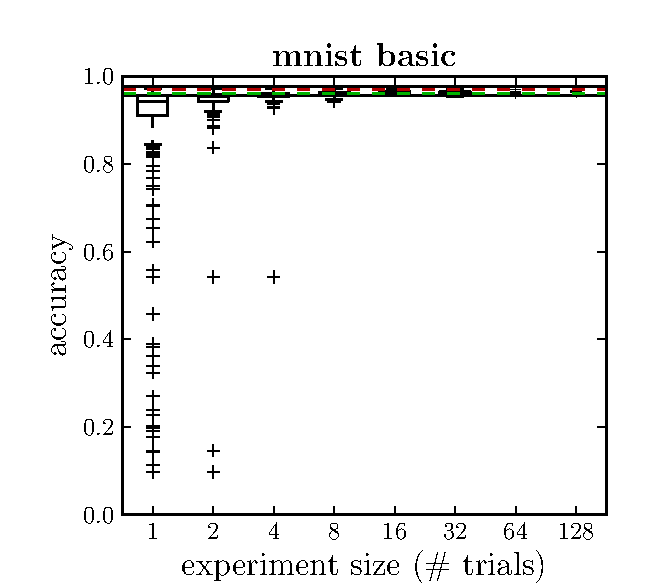
\includegraphics[scale=0.40]{figures/dbn_efficiency/dbn_efficiency_mnist_basic}
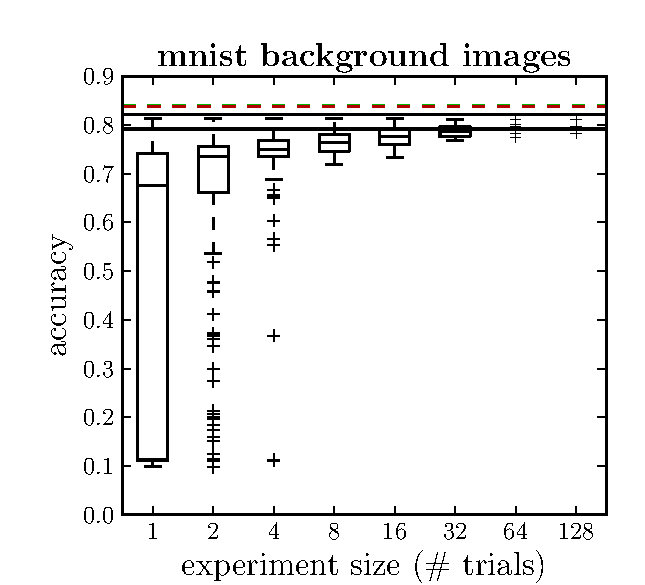
\includegraphics[scale=0.40]{figures/dbn_efficiency/dbn_efficiency_mnist_background_images}
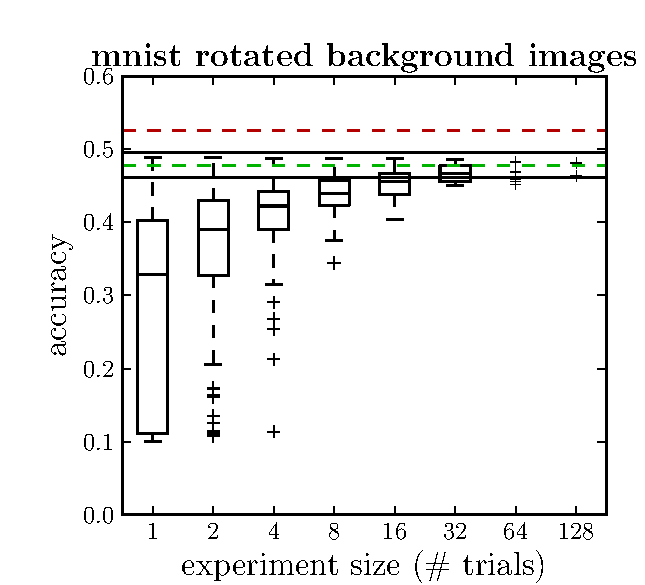
\includegraphics[scale=0.40]{figures/dbn_efficiency/dbn_efficiency_mnist_rotated_background_images}

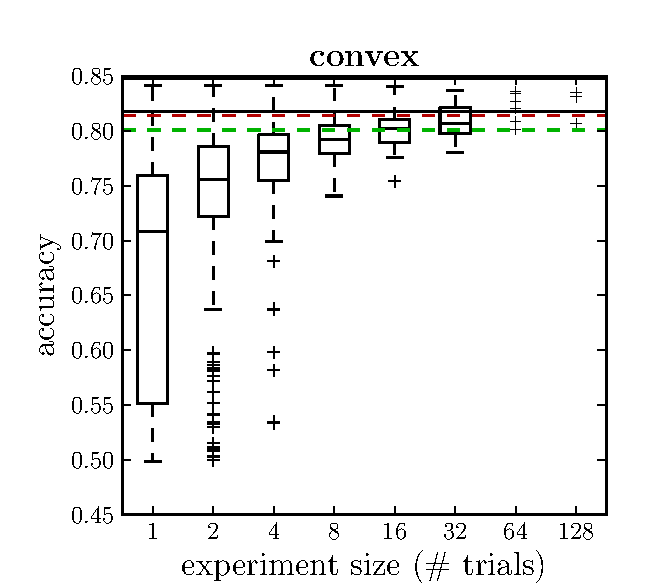
\includegraphics[scale=0.40]{figures/dbn_efficiency/dbn_efficiency_convex}
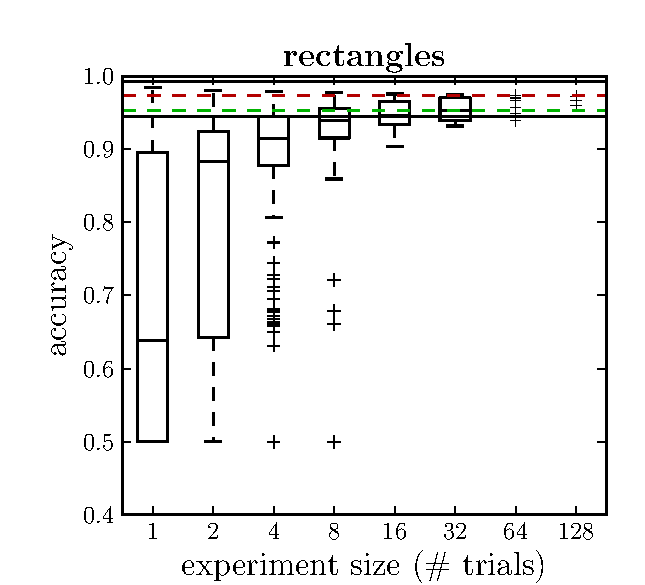
\includegraphics[scale=0.40]{figures/dbn_efficiency/dbn_efficiency_rectangles}
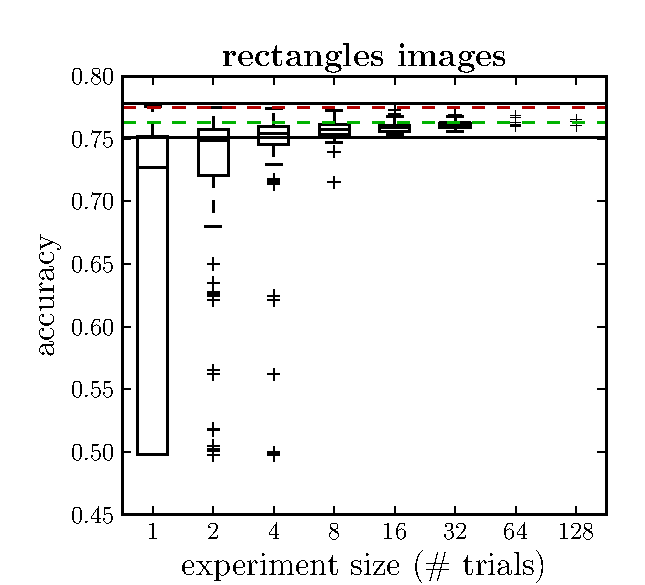
\includegraphics[scale=0.40]{figures/dbn_efficiency/dbn_efficiency_rectangles_images}

\vspace{-1em}

%----------------------------------------
\subsection{Sequential Model-Based Optimization}
%----------------------------------------
\vspace{-1em}

\setlength{\algowidth}{.9\colwidth}
\addtolength{\algowidth}{-0in}

\begin{minipage}[c]{\colwidth}
\begin{tabular}{c}
\begin{algorithm}{$\Algo{SMBO}\big(\text{target } f, \text{model } \blue{M_0},
    \text{Criterion } \red{S}, T \big)$}
\Aitem $\cH \setto \emptyset$,
\Aitem For $t \setto 1$~\To~$T$,
\Aitem \label{ai:candidate}\mt $x^*~\setto~\operatorname{argmin}_{x}~\red{S}(x, \blue{M_{t-1}})$,
\Aitem \mt Evaluate $f(x^*)$, \mt \algoremark{Expensive step}
\Aitem \mt $\cH \setto \cH \cup (x^*,f(x^*))$,
\Aitem \mt \label{ai:update} Fit a new model $\blue{M_t}$ to $\cH$.
\Aitem \Return $\cH$
\end{algorithm}
\end{tabular}
\end{minipage}

Various possible choices for $\red{S}$, including the \un{Expected
  Improvement}.


\columnbreak

%----------------------------------------
\subsection*{Expected Improvement}
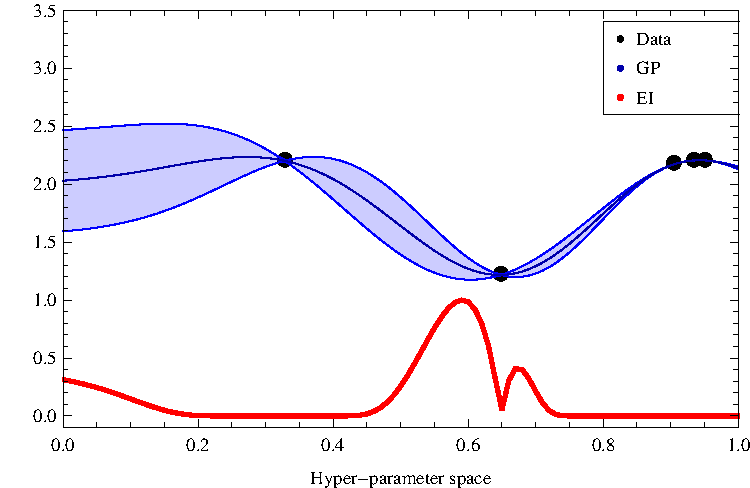
\includegraphics[width = .8\colwidth]{figures/gpei.pdf}




%----------------------------------------
\subsection*{Gaussian Process}
%----------------------------------------

Nested GPs used \un{squared exponential kernels with ARD}:\\

\setlength{\unitlength}{1.1em}
\begin{picture}(50,12.25)(-3, 2)
%\put(-3, 15.25){ \makebox(0,0)[l]{RANDOM CONFIGURATION:}}

\put(0, 14){ \makebox(0,0)[l]{ZCA ?}}
\put(6, 14){ \vector(1, 0){1.5}}
\put(8, 14){ \makebox(0,0)[l]{ZCA energy}}

\put(0, 13){ \makebox(0,0)[l]{layer1.n\_hid}}
\put(0, 12){ \makebox(0,0)[l]{layer1.cd\_lr}}
\put(0, 11){ \makebox(0,0)[l]{...}}
\put(0, 10){ \makebox(0,0)[l]{layer1.cd\_epochs}}

\put(0, 9){ \makebox(0,0)[l]{layer2 ?}}
\put(6, 9){ \vector(1, 0){1.5}}
\put(8, 9){ \makebox(0,0)[l]{layer2.n\_hid}}
\put(8, 8){ \makebox(0,0)[l]{layer2.cd\_lr}}
\put(8, 7){ \makebox(0,0)[l]{...}}
\put(8, 6){ \makebox(0,0)[l]{layer2.cd\_epochs}}

\put(8, 5){ \makebox(0,0)[l]{layer3 ?}}
\put(14, 5){ \vector(1, 0){1.5}}
\put(16, 5){ \makebox(0,0)[l]{layer2.n\_hid}}
\put(16, 4){ \makebox(0,0)[l]{layer2.cd\_lr}}
\put(16, 3){ \makebox(0,0)[l]{...}}
\put(16, 2){ \makebox(0,0)[l]{layer2.cd\_epochs}}

\color{darkgreen}
\put(2.75, 11.5) { \oval(7.75, 7) }
\put(10.75, 7.5) { \oval(7.75, 7) }
\put(18.75, 3.5) { \oval(7.75, 7) }

\put(10.75, 14.0) { \oval(7.75, 2) }

%\put(14, 7){ \vector(1, 0){2}}
%\put(0, 6){ \makebox(0,0)[l]{layer1.n\_hid}}
%\put(0, 5){ \makebox(0,0)[l]{layer1.n\_hid}}
%\put(0, 4){ \makebox(0,0)[l]{layer1.n\_hid}}
%\put(0, 3){ \makebox(0,0)[l]{layer1.n\_hid}}
%\put(0, 2){ \makebox(0,0)[l]{layer1.n\_hid}}
%\put(0, 1){ \makebox(0,0)[l]{layer1.n\_hid}}
\end{picture}


%----------------------------------------
\subsection*{Tree-structured Parzen Estimator (TPE)}
%----------------------------------------
\begin{minipage}{\linewidth}
Construct densities for \un{good} and \un{bad} hyper-parameter regions by replacing
sampling distributions with \un{Parzen / Multinomial} densities:
\begin{itemize}
\setlength{\itemsep}{0pt}
\setlength{\parsep}{0pt}
\item $\ell(h) = \prod_i \mathrm{Parzen}(h_i ~|~ h' \in \mathcal{H}: f(h') < \gamma)$
    models region with $f$ \un{better} than $\gamma$
\item $g(h) = \prod_i \mathrm{Parzen}(h_i ~|~ h' \in \mathcal{H}: f(h') \geq
\gamma)$
    models region with $f$ \un{worse} than $\gamma$
\begin{equation*}
    \operatorname*{argmax}_{\mathrm{config}} ~ \mathrm{EI}(\mathrm{config}) =
    \operatorname*{argmax}_{\mathrm{config}} ~ \frac{\ell(\mathrm{config})}{g(\mathrm{config})}
\end{equation*}
\item \un{Training and approx. maximization are fast}: $O(n\log n)$ in
  $|\mathcal{H}|$
\end{itemize}
\end{minipage}

%\vspace*{-3mm}
\subsection{Optimizing Expected Improvement}

\vspace{-.5em}
Hardest datasets for random search: {\bf 1) convex}, {\bf 2) mnist rotated background images}.

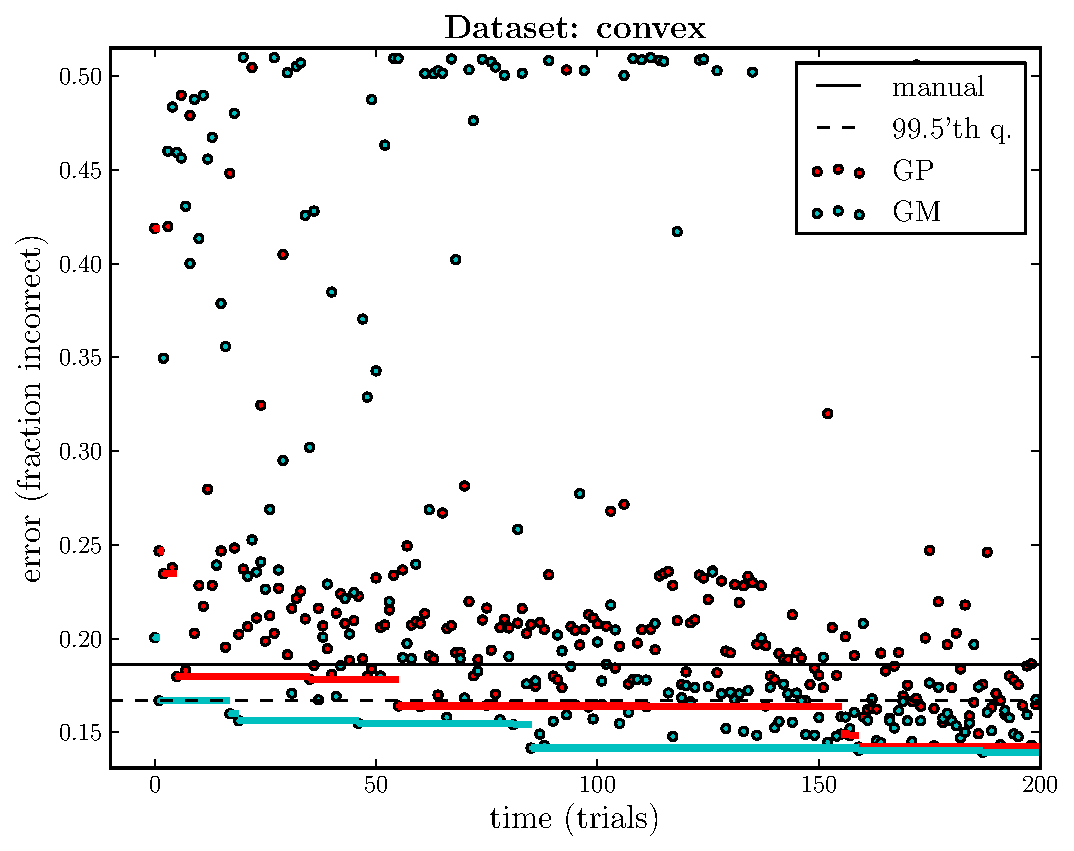
\includegraphics[scale=.365]{figures/plot_histories_gp3,gm_convex.pdf}
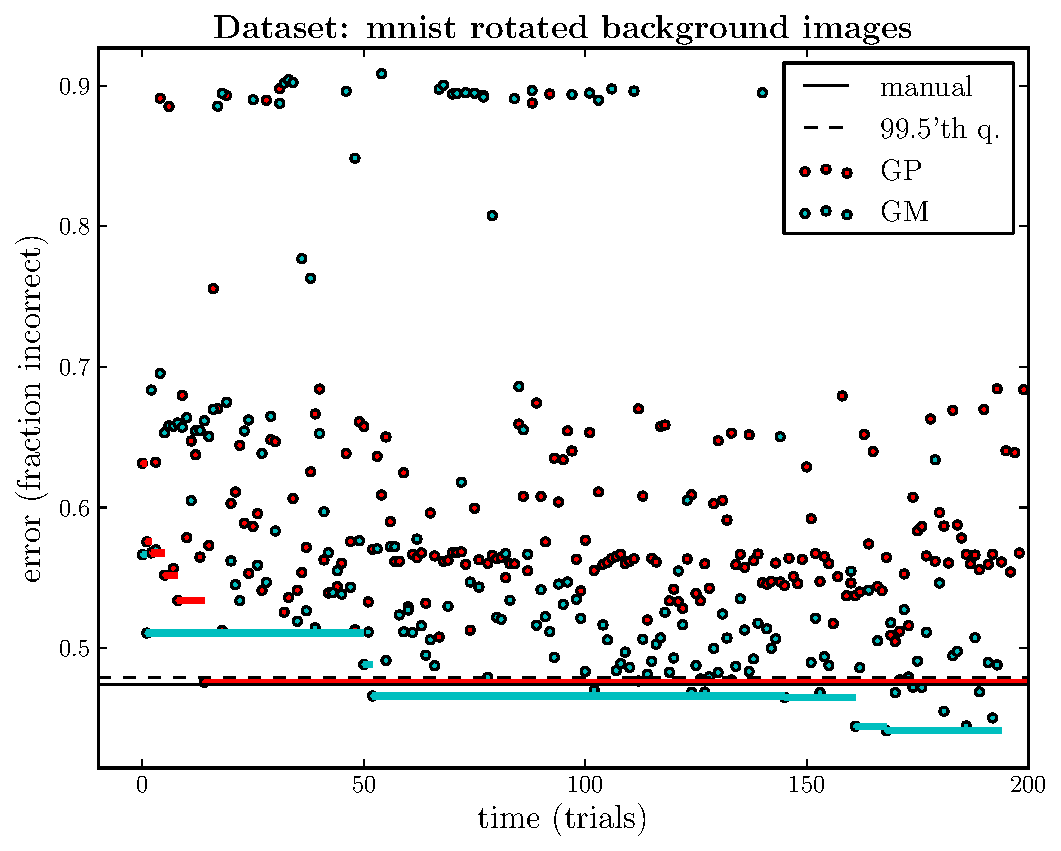
\includegraphics[scale=.365]{figures/plot_histories_gp3,gm_mnist_rotated_background_images.pdf}

%\vspace*{-3mm}
Hyper-optimization worked better than manual, and TPE outperformed GP.
\onecol

\end{document}

\subsection{Conclusions}

\begin{itemize}
    \setlength{\itemsep}{0pt}
    \setlength{\parsep}{0pt}
    \setlength{\topsep}{0pt}
    \setlength{\partopsep}{0pt}
    % XXX: wherefore does nothing work here??
    \item Random search is competitive with sequential manual + grid search.
    \item In hard problems, if budget allows \# trials $> 50$ then EI optimization is worthwhile.
    \item Hyper-parameter optimization has discovered new best results on these datasets.
    \item Sequential optimization can be parallelized to a certain extent (e.g.
        5-10 nodes).
    \item TPE implemented in ``Hyperopt'': \texttt{https://github.com/jaberg/hyperopt}
\end{itemize}

\begin{table}
\vs{4}
    \caption{Distribution over DBN hyper-parameters for random sampling.
    Options separated by ``or''  such as pre-processing (and including the random seed) are weighted equally.
    Symbol $U$ means uniform, $\mathcal{N}$ means Gaussian-distributed, and $\log U$ means uniformly distributed in the log-domain.
    CD (also known as CD-1) stands for contrastive divergence, the algorithm used to initialize the layer parameters of the DBN.
    %and the distribution used by the \algorandom\ algorithm.
    }
    \label{tbl:dbnprior}
    \centering
\vs{4}
\end{table}

    %\caption
    %{Deep Belief Network (DBN) performance according to random search.
    %Random search is used to explore up to 32 hyper-parameters (see Table~\ref{tbl:dbnprior}).
    %Results found using a grid-search-assisted manual search over a similar domain with
    %an average 41 trials are given in green (1-layer DBN) and red (3-layer DBN).
    %Each box-plot (for $N=1,2,4,...)$ shows the distribution of test set performance when the best model among
    %$N$ random trials is selected. The datasets ``convex'' and ``mnist rotated
    %background images'' are used for more thorough hyper-parameter
    %optimization.
    %}
    %\label{fig:dbn_random_efficiency}

\begin{figure}
\centering
\begin{minipage}{0.9\linewidth}
% /home/bergstra/cvs/hyperopt/hyperopt/dbn.py plot_histories mongo://localhost:20111/dbn_%s_%s/jobs gp3,gm convex 0 2000
  \vs{0}
  \vs{6}
% /home/bergstra/cvs/hyperopt/hyperopt/dbn.py plot_histories mongo://localhost:20111/dbn_%s_%s/jobs gp3,gm mnist_rotated_backgound_images 0 2000
    \caption{Efficiency of Gaussian Process-based (GP) and graphical
    model-based (TPE) sequential optimization algorithms on the task of optimizing the validation set performance of a DBN of up to three layers on the {\bf convex} task (left) and the {\bf MRBI} task (right).
    The dots are the elements of the trajectory $\cH$ produced by each SMBO algorithm.
    The solid coloured lines are the validation set accuracy of the best trial found before each point in time.
    Both the TPE and GP algorithms make significant advances from their random
    initial conditions, and substantially outperform the manual and random
    search methods. A 95\% confidence interval
    about the best validation means on the {\bf convex} task extends 0.018 above and below each point,
    and on the {\bf MRBI} task extends 0.021 above and below each point.
    The solid black line is the test set accuracy obtained by domain experts using a combination
    of grid search and manual search~\citep{Larochelle+etal:2007}.
    The dashed line is the 99.5\% quantile of validation performance found among trials sampled from our prior distribution (see Table~\ref{tbl:dbnprior}),
    estimated from 457 and 361 random trials on the two datasets respectively.
    % convex has n=1500 validation points
    % best scores have Bernoulli param p = 0.15
    % variance is 1.96 sqrt(p * (1-p)/n) = 0.018%
    % MRBI has n=2000 validation points, p=.45
    }
  \vs{4}
    \label{fig:H}
\end{minipage}
\end{figure}

\section{Conclusions}

Future work includes
\vspace{-0.4cm} 
\begin{itemize}
\item bla
\end{itemize}

